% Created 2016-05-14 Sam 19:59
\documentclass[11pt, a4paper]{article}
\usepackage[utf8]{inputenc}
\usepackage[T1]{fontenc}
\usepackage{fixltx2e}
\usepackage{graphicx}
\usepackage{longtable}
\usepackage{float}
\usepackage{wrapfig}
\usepackage{soul}
\usepackage{textcomp}
\usepackage{marvosym}
\usepackage{wasysym}
\usepackage{latexsym}
\usepackage{amssymb}
\usepackage{hyperref}
\tolerance=1000
\usepackage{minted}
\usepackage[utf8]{inputenc}
\usepackage[english]{babel}
\usepackage{graphicx}
\usepackage[left=2.35cm, right=3.35cm, top=3.35cm, bottom=3.0cm]{geometry}
\usepackage{titling}
\providecommand{\alert}[1]{\textbf{#1}}

\title{Statistical methods for bioinformatics \linebreak GAM and Trees}
\author{Cedric Lood}
\date{\today}
\hypersetup{
  pdfkeywords={},
  pdfsubject={},
  pdfcreator={Emacs Org-mode version 7.9.3f}}

\begin{document}

\maketitle


\graphicspath{ {figures/} }
\setlength{\droptitle}{-5em} 
\setlength{\parindent}{0cm}

\section{Applied exercises}
\label{sec-1}
\subsection{Question 10}
\label{sec-1-1}

Libraries and definition of the training and test sets used for the
analysis:

\begin{minted}[]{R}
library(ISLR)
library(boot)
library(ggplot2)
library(leaps)
library(gam)

attach(College)
set.seed(1)
train <- sample(c(TRUE,FALSE), nrow(College), rep=TRUE)
test <- (!train)
\end{minted}
\subsubsection{Part a}
\label{sec-1-1-1}

The analysis reveals a forward selection with 6 variables retained in
the model:


\begin{minted}[]{R}
model.fwd <- regsubsets(Outstate~.,data=College[train,], nvmax=17,method="forward")
test.mat <- model.matrix(Outstate~., data=College[test,])

val.errors <- rep(NA, 17)
for(i in 1:17){
    coefi <- coef(model.fwd, id=i)
    pred <- test.mat[,names(coefi)] %*% coefi
    val.errors[i] <- mean((College$Outstate[test]-pred)^2)
}
val.errors
which.min(val.errors)
coef(model.fwd, 6)
\end{minted}


\begin{verbatim}
> val.errors
 [1] 10734659  7647452  6468424  5434378  4948421  4650921  4734848  4718857
 [9]  4690641  4735896  4694172  4877469  4754741  4690085  4711840  4700313
[17]  4700869
> which.min(val.errors)
[1] 6
> coef(model.fwd, 6)
  (Intercept)    PrivateYes    Room.Board      Terminal   perc.alumni 
-4227.6797221  2778.7052614     0.8106532    49.5653264    38.3960635 
       Expend     Grad.Rate 
    0.2616141    26.3975500
\end{verbatim}
\subsubsection{Part b}
\label{sec-1-1-2}

For this section, there are potentially many different GAM that could
be produced. For example, one could produce different functionals
consisting of smoothing splines for each of the predictors, with
different combinations of degrees of freedom. Here are a few, the
first one being akin to a multiple linear regression:


\begin{minted}[]{R}
model.gam <- gam(Outstate~Private+Room.Board+Terminal+perc.alumni+Expend+Grad.Rate,data=College[train,])
pdf("gam_trees_s.pdf", width=16, height=12)
par(mfrow = c(3, 2))
plot.gam(model.gam,se=TRUE,col="green")
dev.off()

model.gam.s2 <- gam(Outstate~Private+s(Room.Board,df=2)+s(Terminal,df=2)+s(perc.alumni,df=2)+s(Expend,df=2)+s(Grad.Rate,df=2),data=College[train,])
pdf("gam_trees_s_2.pdf", width=16, height=12)
par(mfrow = c(3, 2))
plot.gam(model.gam.s,se=TRUE,col="green")
dev.off()

model.gam.s.3 <- gam(Outstate~Private+s(Room.Board,df=3)+s(Terminal,df=3)+s(perc.alumni,df=3)+s(Expend,df=3)+s(Grad.Rate,df=3),data=College[train,])
pdf("gam_trees_s_3.pdf", width=16, height=12)
par(mfrow = c(3, 2))
plot.gam(model.gam.s.3,se=TRUE,col="green")
dev.off()
\end{minted}

The graphics for the other 2 models can be found in the annex. Here
is the one for the smoothing splines with 2 degrees of freedom: 

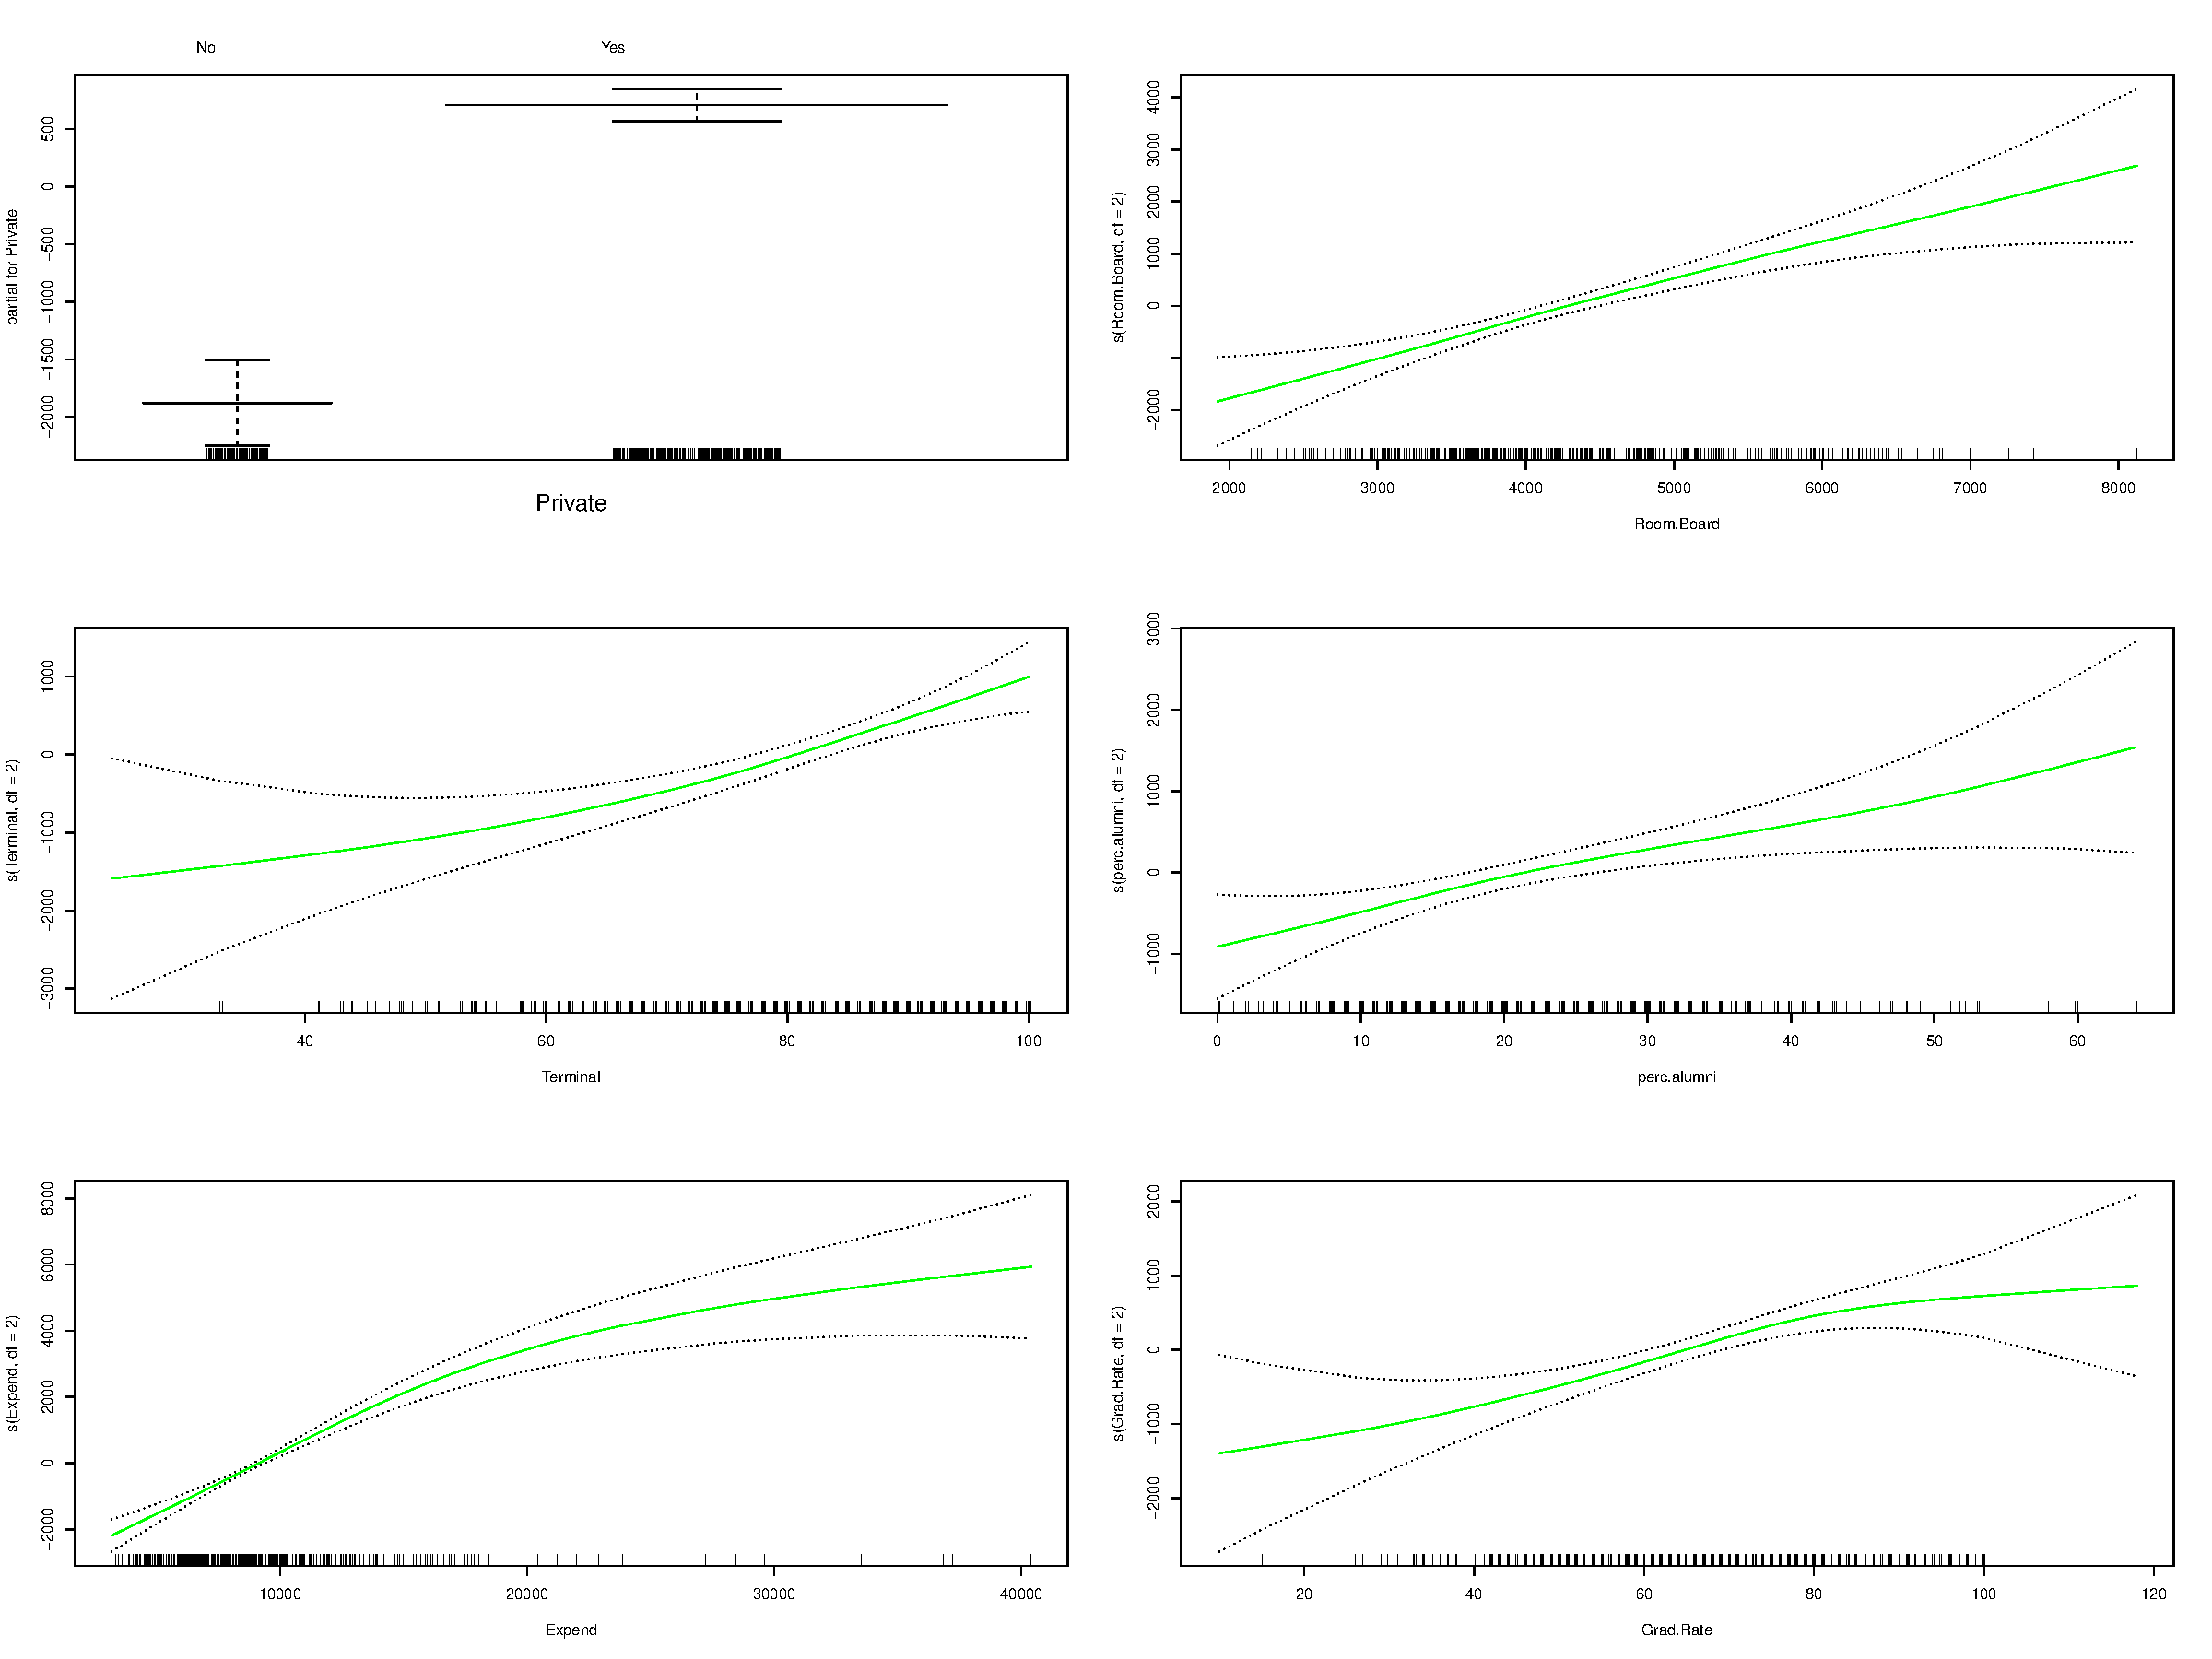
\includegraphics[scale=0.45]{gam_trees_s_2.pdf}
\subsubsection{Part c}
\label{sec-1-1-3}

This is the evaluation of the 3 different models for the test sets,
followed by the results. 


\begin{minted}[]{R}
gam.pred <- predict(model.gam,College[test,])
gam.err <- mean((College[test,]$Outstate - gam.pred)^2)

gam.pred.s2 <- predict(model.gam.s2,College[test,])
gam.err.s2 <- mean((College[test,]$Outstate - gam.pred.s2)^2)

gam.pred.s3 <- predict(model.gam.s.3,College[test,])
gam.err.s3 <- mean((College[test,]$Outstate - gam.pred.s3)^2)
\end{minted}


\begin{verbatim}
> gam.err
[1] 4650921
> gam.err.s2
[1] 3952853
> gam.err.s3
[1] 3784922
\end{verbatim}
\subsubsection{Part d}
\label{sec-1-1-4}

Evidence of non-linear relationship between variables can be
investigated using the summary function on the GAM. The function
provides the user with a non-parametric ANOVA table. Below is the
output of the command, which seem to indicate a non-linear
relationship between the predictor ``Expend'' and the dependent
value. 


\begin{verbatim}
> summary(model.gam.s2)

Call: gam(formula = Outstate ~ Private + s(Room.Board, df = 2) + s(Terminal, 
    df = 2) + s(perc.alumni, df = 2) + s(Expend, df = 2) + s(Grad.Rate, 
    df = 2), data = College[train, ])
Deviance Residuals:
    Min      1Q  Median      3Q     Max 
-7045.4 -1145.4    84.8  1184.1  5047.0 

(Dispersion Parameter for gaussian family taken to be 3452101)

    Null Deviance: 6006262152 on 405 degrees of freedom
Residual Deviance: 1360128366 on 394.0002 degrees of freedom
AIC: 7278.121 

Number of Local Scoring Iterations: 2 

Anova for Parametric Effects
                        Df     Sum Sq    Mean Sq F value    Pr(>F)    
Private                  1 1635387248 1635387248 473.737 < 2.2e-16 ***
s(Room.Board, df = 2)    1 1343549886 1343549886 389.198 < 2.2e-16 ***
s(Terminal, df = 2)      1  597441375  597441375 173.066 < 2.2e-16 ***
s(perc.alumni, df = 2)   1  240771844  240771844  69.746 1.161e-15 ***
s(Expend, df = 2)        1  424246993  424246993 122.895 < 2.2e-16 ***
s(Grad.Rate, df = 2)     1   63996091   63996091  18.538 2.104e-05 ***
Residuals              394 1360128366    3452101                      
---
Signif. codes:  0 ‘***’ 0.001 ‘**’ 0.01 ‘*’ 0.05 ‘.’ 0.1 ‘ ’ 1

Anova for Nonparametric Effects
                       Npar Df  Npar F     Pr(F)    
(Intercept)                                         
Private                                             
s(Room.Board, df = 2)        1  0.5670    0.4519    
s(Terminal, df = 2)          1  2.2148    0.1375    
s(perc.alumni, df = 2)       1  1.0512    0.3059    
s(Expend, df = 2)            1 26.1955 4.837e-07 ***
s(Grad.Rate, df = 2)         1  3.5803    0.0592 .  
---
Signif. codes:  0 ‘***’ 0.001 ‘**’ 0.01 ‘*’ 0.05 ‘.’ 0.1 ‘ ’ 1
\end{verbatim}
\subsection{Trees Vijver}
\label{sec-1-2}
\subsubsection{Performance with Ridge and Lasso}
\label{sec-1-2-1}

For reminder, here are the performance obtained using regularization
techniques:


\begin{verbatim}
> perf.ridge
[1] 0.6489362
\end{verbatim}


\begin{verbatim}
> perf.lasso
[1] 0.6170213
\end{verbatim}
\subsection{Annex}
\label{sec-1-3}

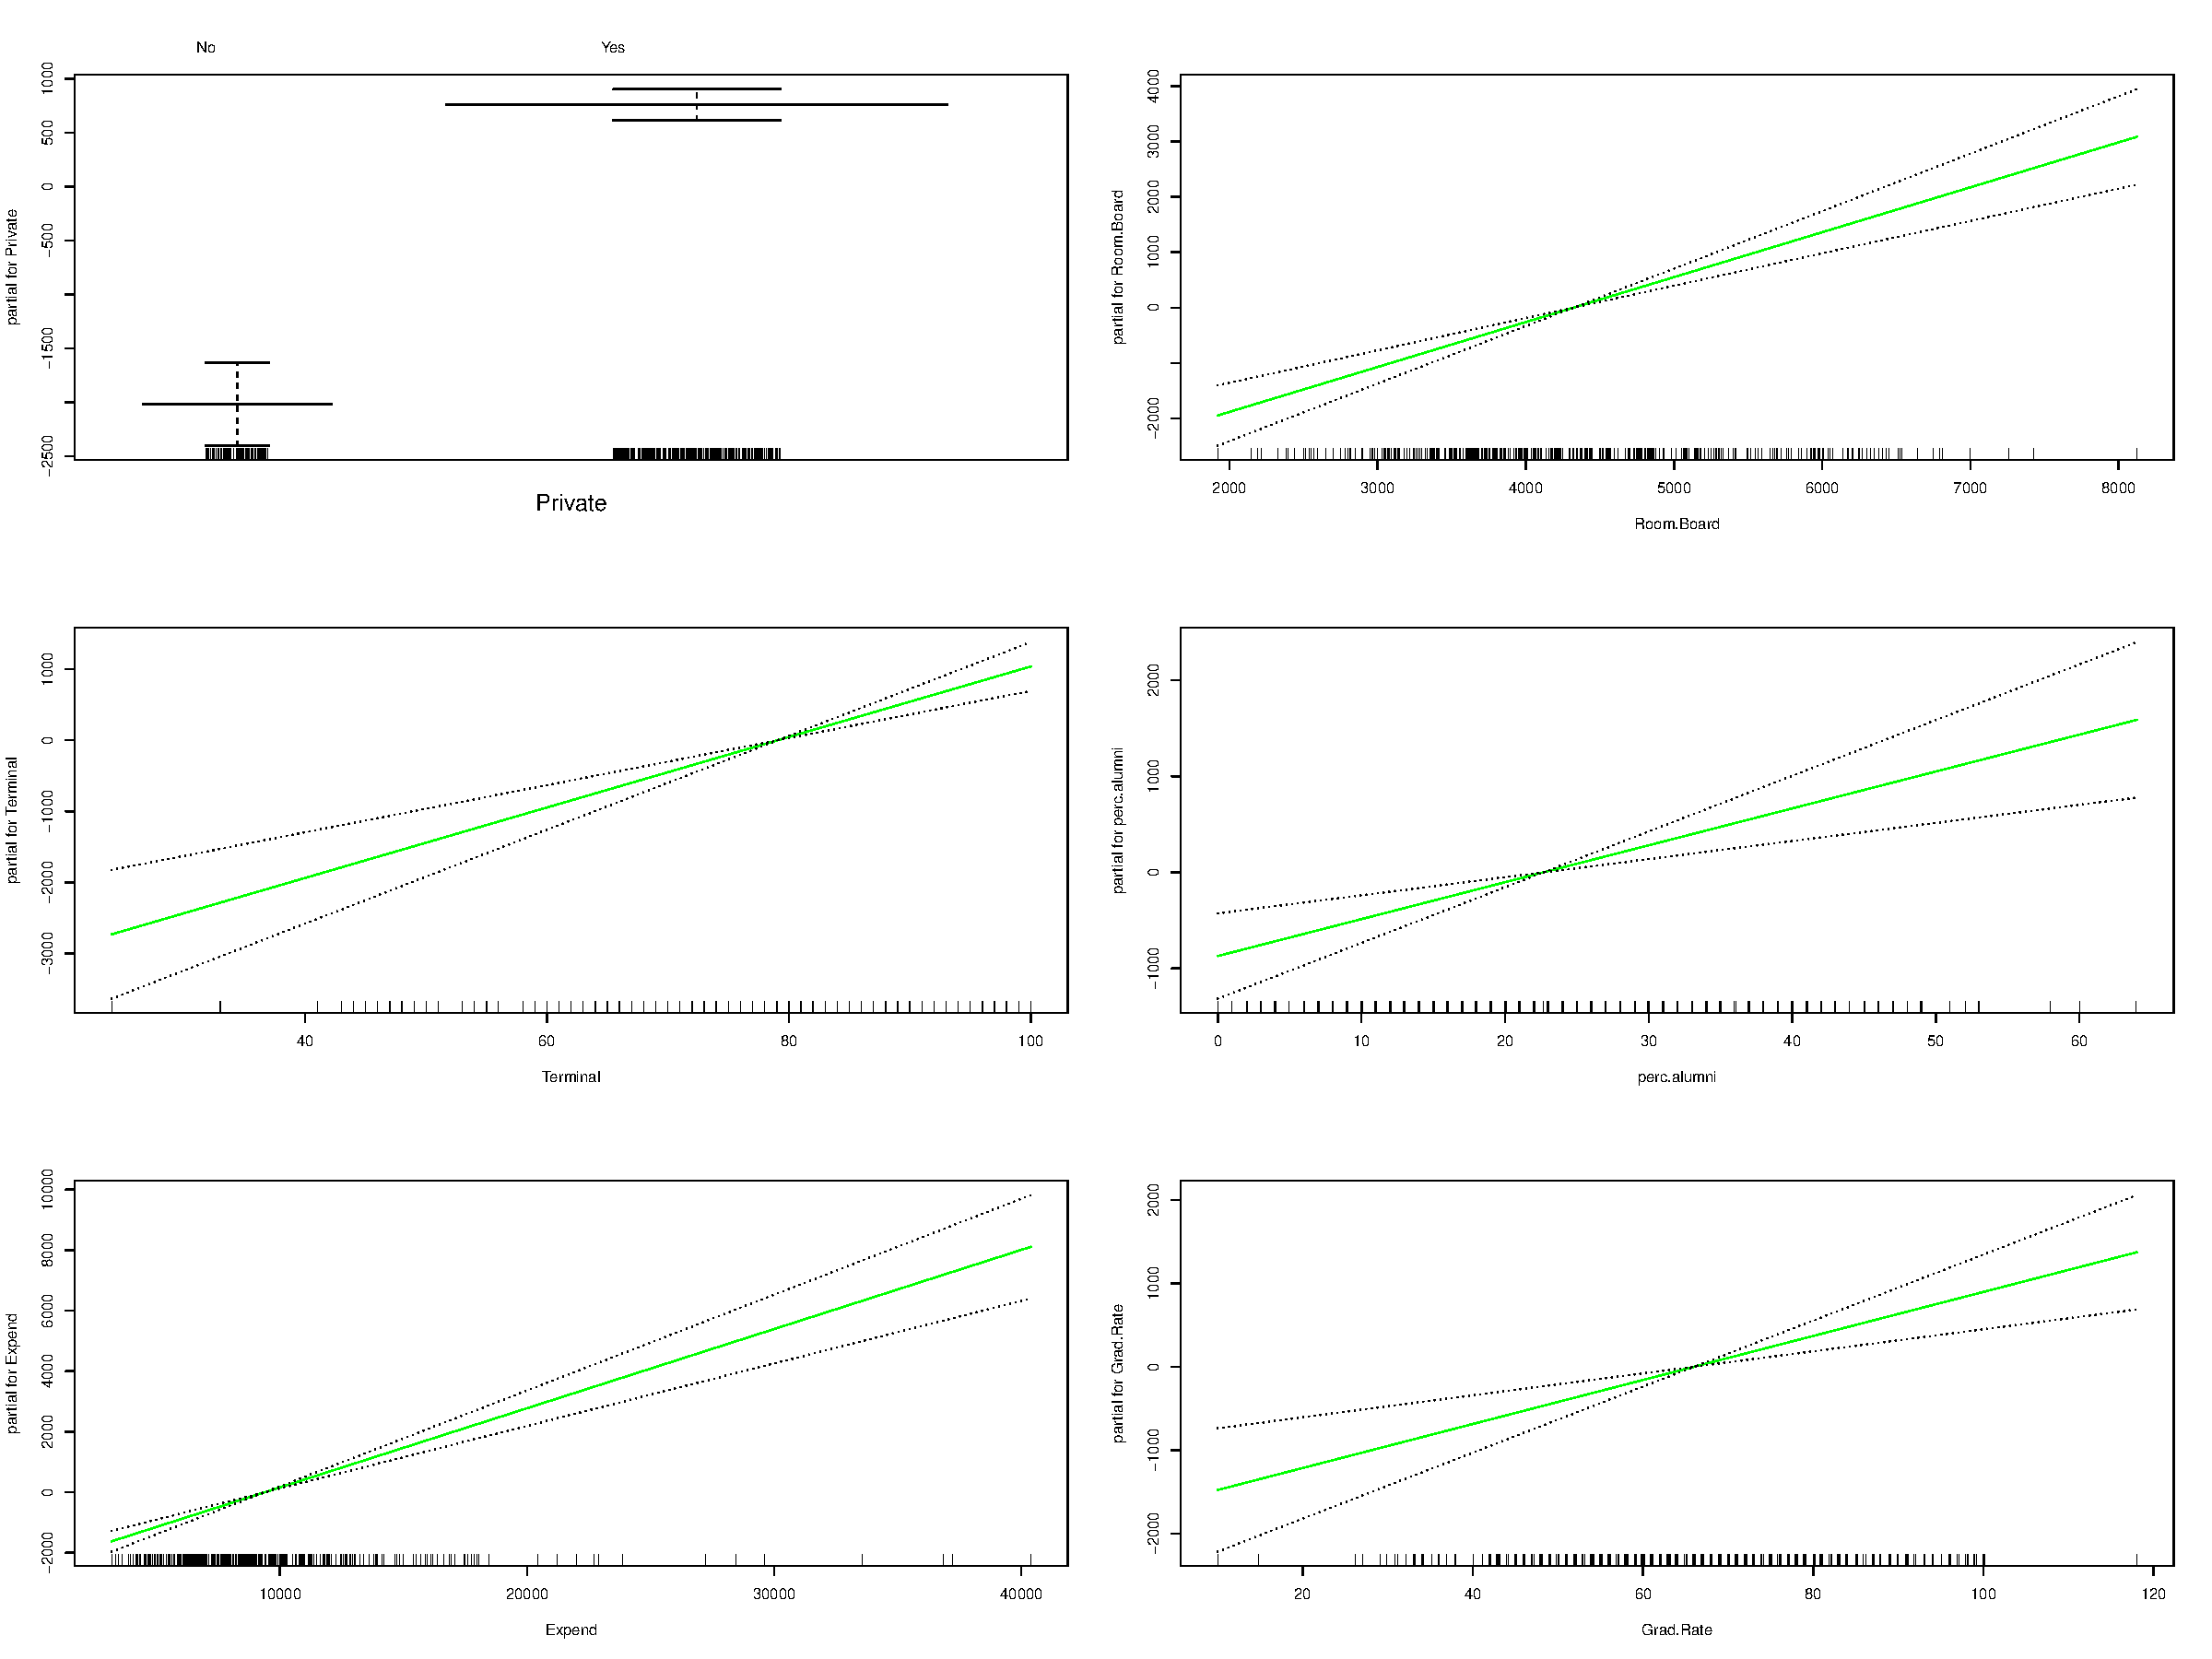
\includegraphics[scale=0.4]{gam_trees_s.pdf}

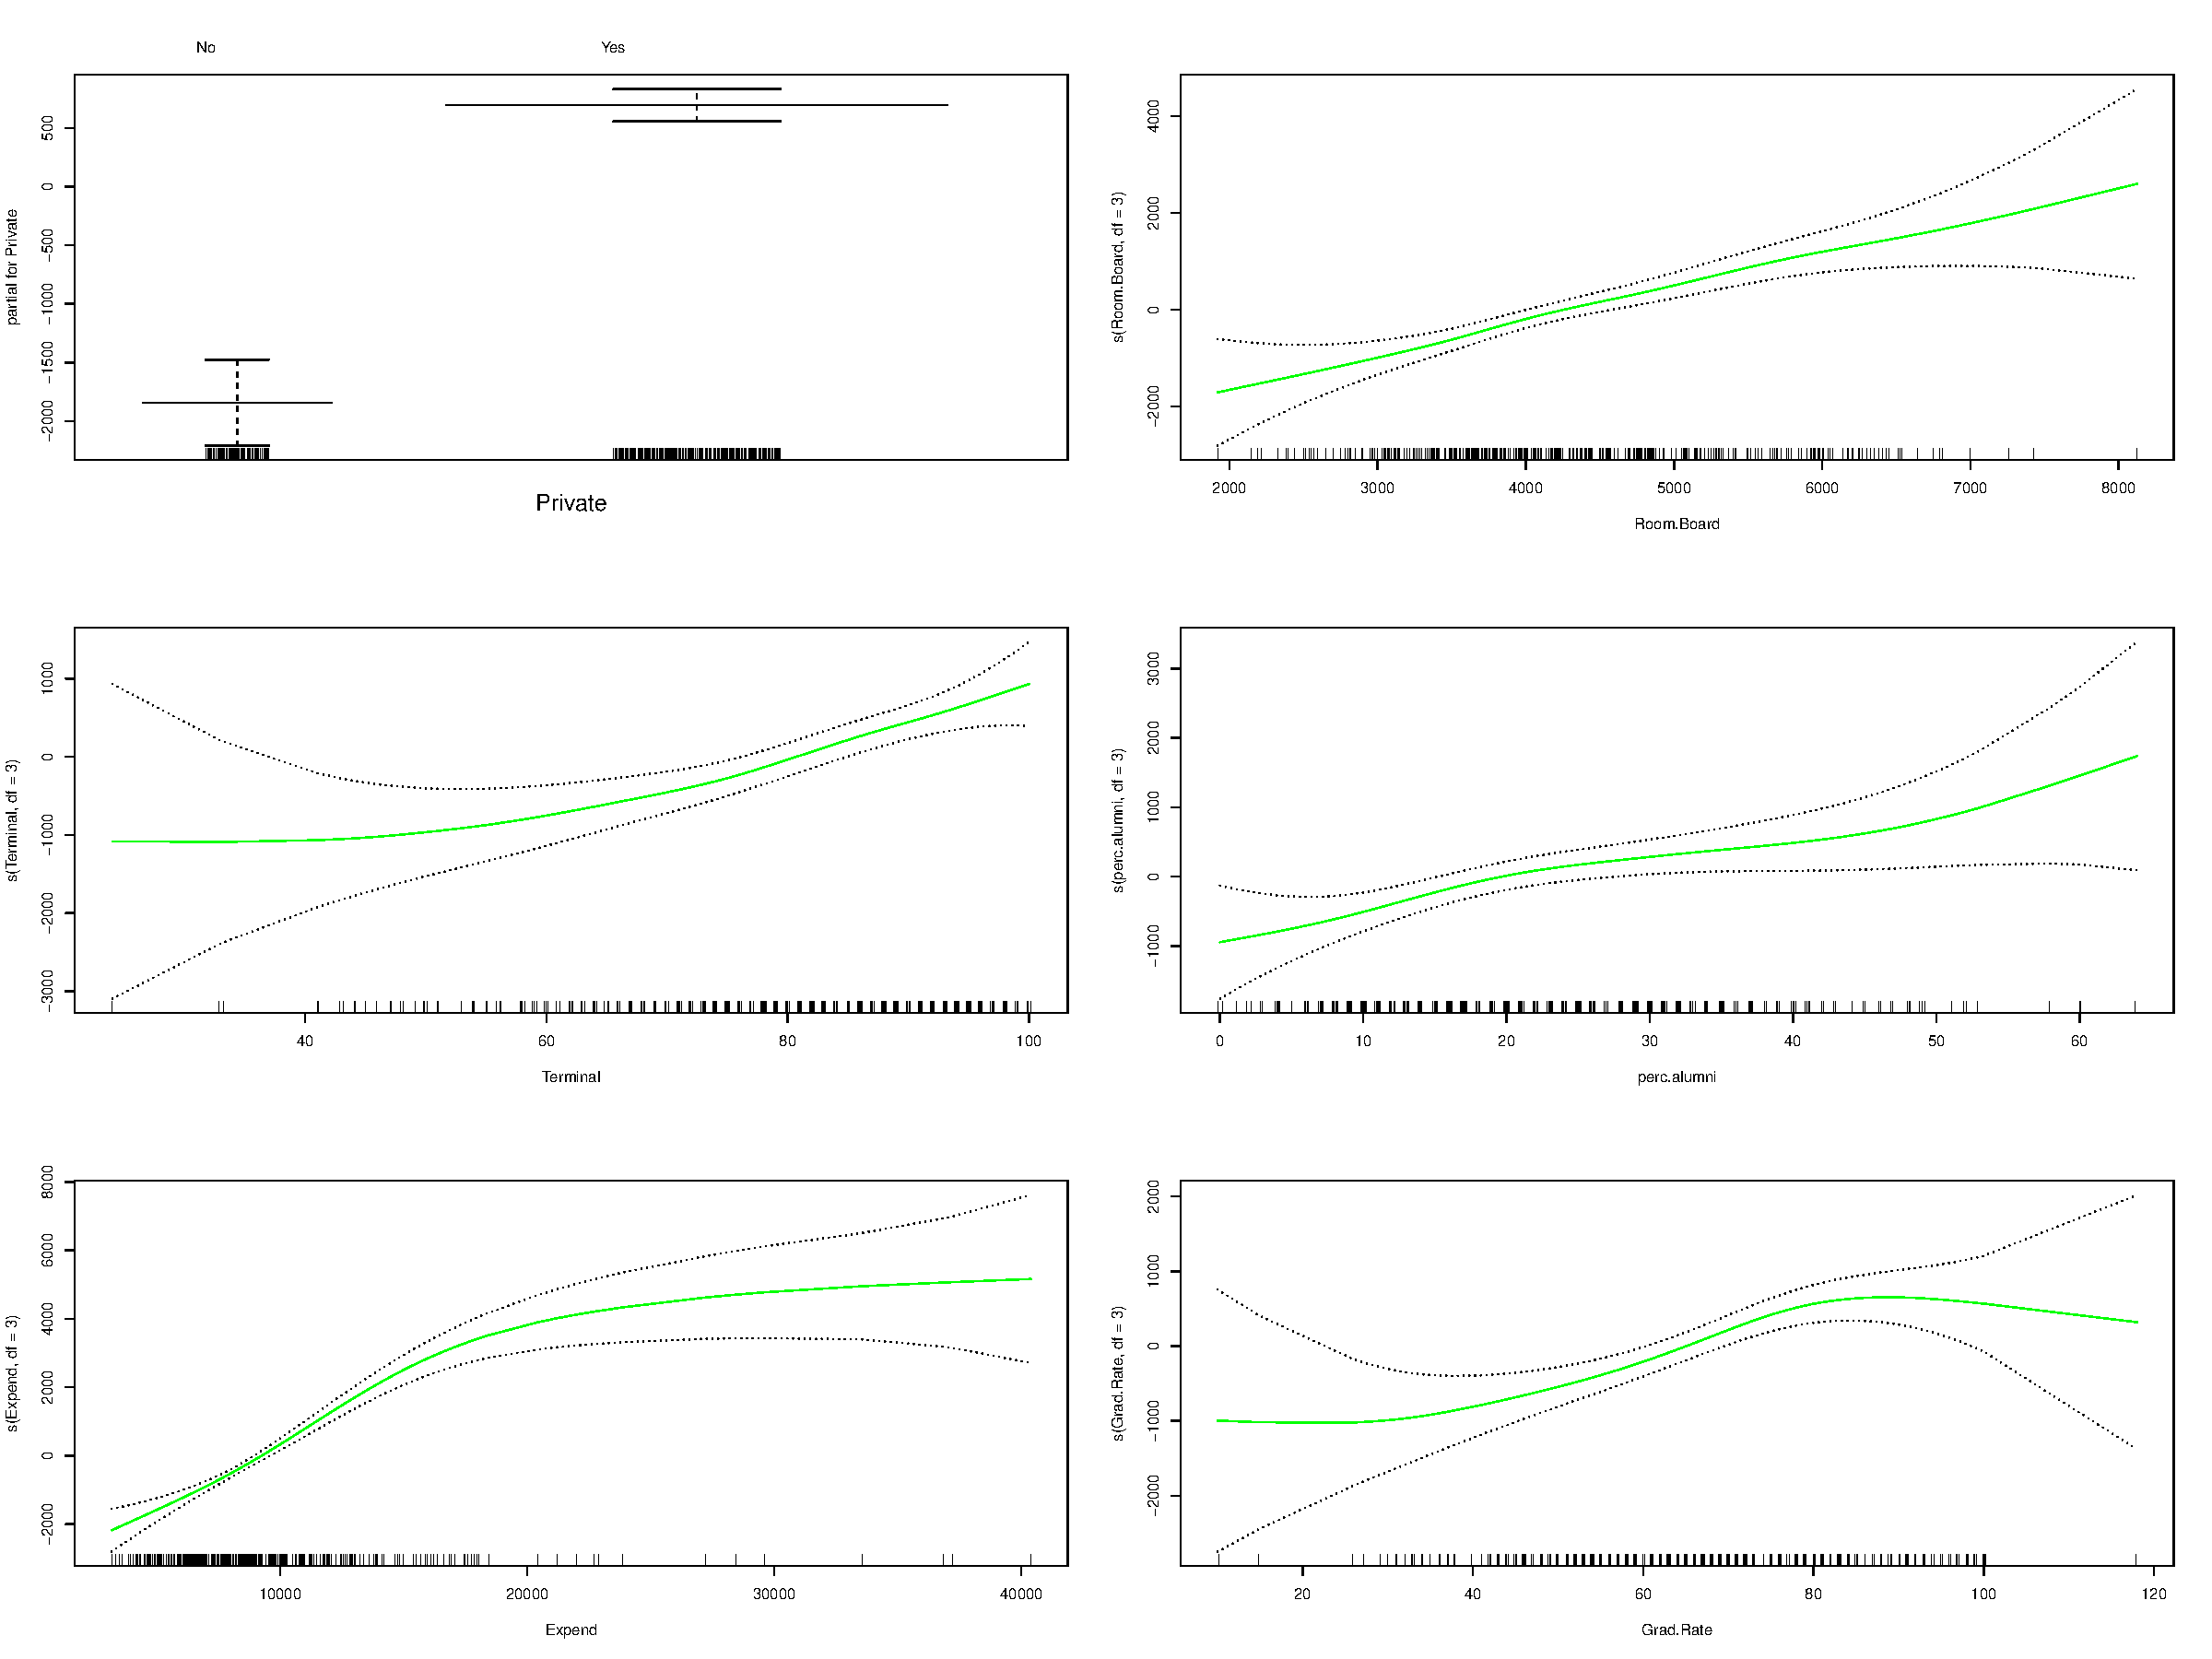
\includegraphics[scale=0.4]{gam_trees_s_3.pdf}

\end{document}
